\chapter{From an observable correlation to necessary dissipation}
\label{pa:entry}
A stationary scalar autocorrelation looks the same when time is reversed.
It can nevertheless rule out every reversible hidden Markov explanation
within a declared physical class. The reason is that reversible semigroups
impose relations between correlations at different lags. This chapter develops
a direct quantitative use of that constraint.

Let $f$ be a bounded instantaneous observable of a stationary Markov process,
$C(t)=\mathbb E[f(X_0)f(X_t)]$, and let $R$ bound the range of $f$.
For a chosen real $s$, define
\[
 \Delta_s=-s^2 C(0)+2s C(t)-C(2t).
\]
The following chapter proves that, under ordinary reversal of the full hidden
state and the stated path-entropy contract,
\[
 \sigma\geq\frac{1}{t}\,
 \phi\!\left(\frac{4[\Delta_s]_+}{R^2}\right),
 \qquad \phi(u)=2\sqrt u\operatorname{artanh}\sqrt u\geq2u.
\]
The finite expression applies for $0\leq u<1$. Its linear consequence is
$\sigma\geq8[\Delta_s]_+/(R^2t)$. No hidden-state reconstruction is required
for this implication. The assumptions still concern the hidden process:
an even recorded observable does not establish the required reversal rule.

This result improves the conversion of a covered correlation contrast into a
physical lower bound. It does not increase the statistical evidence in the
record. Replaying the sixth edition's frozen driven example, with no change to
its records or confidence event, raises the mean certified rate from
$0.0008005133$ to $0.11224493$, a factor of $140.216$. The actual simulated
rate is $3.55736$, so the remaining gap is substantial. Detection remains
$399/400$: the improvement is quantitative, not a larger number of discoveries.

The next chapters supply a usable acquisition scheme. Bounded analog readings
provide both lagged products and a conservative zero-lag calibration from
squared readings. One joint confidence contrast accounts for their sampling
uncertainty. In a separate frozen simulated experiment at identical data and
resources, this joint method produces $399/400$ positive certificates versus
$377/400$ for the earlier split-calibration analog method. The experiment uses
$16{,}000$ scalar detector readings and $900$ units of evolution time per
replicate. Preparation and detector energy need additional calibration.

The noisy failure then motivates a new experiment. Exact calculation shows
that the earlier two-lag family has no positive population witness, while a
predeclared later lag does. On fresh noisy records, retiming restores
$386/400$ positive certificates versus $0/400$ for both earlier fixed
contrasts. It uses the same $900$ units of evolution time and $3{,}600$
readings instead of $16{,}000$. This changes experimental access; it is not
a reanalysis of the same acquired records or a universal timing prescription.

There are three different optimization problems here:
\begin{enumerate}
\item Optimize a lower bound on a discrepancy between observed laws.
\item Minimize physical entropy over all hidden models compatible with those laws.
\item Minimize it within a specified physical architecture.
\end{enumerate}
The first does not automatically solve the second. An exact finite-size
circulant calculation solves a version of the third and supplies realizable
comparison systems. A sampling theorem also shows why, even with perfect
spatial resolution, a finite menu of time gaps cannot generally provide a
finite upper bound on dissipation without further restrictions.

\begin{figure}[ht]
\centering
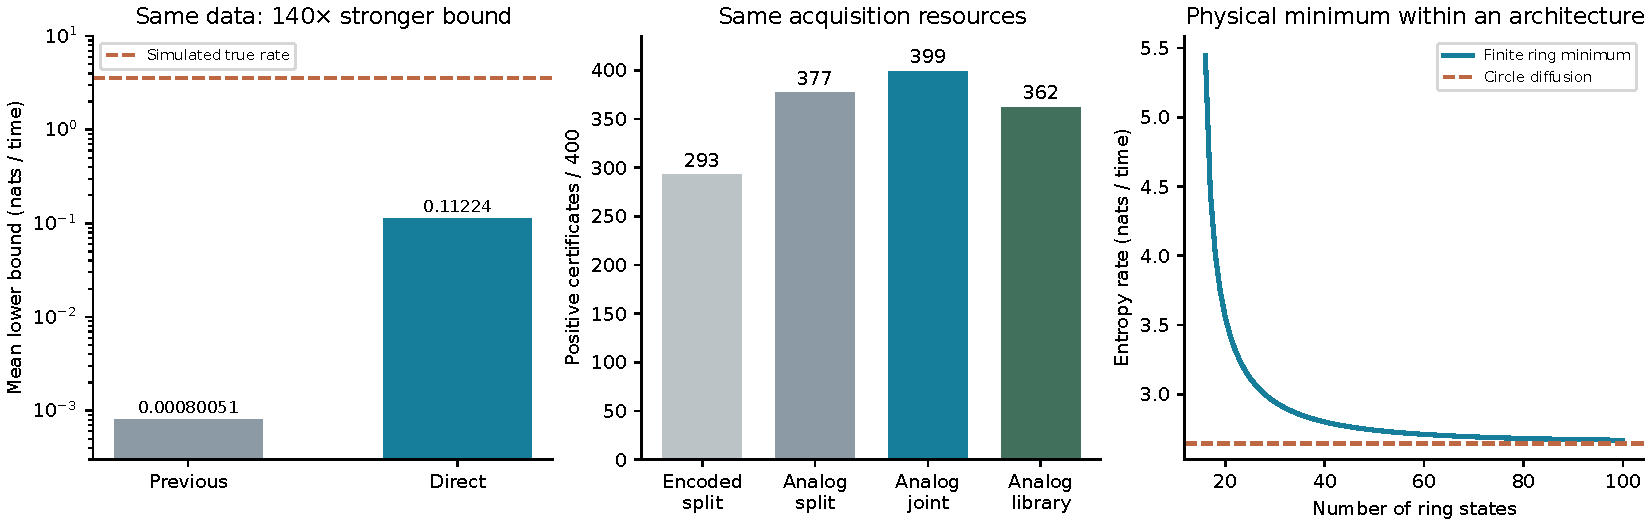
\includegraphics[width=\textwidth]{figures/attainability.pdf}
\caption{Distinct meanings of improvement. Left: the new physical bridge
strengthens a lower bound using the same frozen observations. Middle: joint
analog confidence increases detection at matched acquisition cost; selecting
from a library pays an explicit statistical penalty. Right: physically
realizable ring minima approach the known circle value inside a specified
architecture. All numerical panels describe mathematical models and simulated
records, not new laboratory measurements.}
\label{fig:pa-overview}
\end{figure}

For practical use, start with the acquisition contract in the joint analog
chapter and the executable \texttt{attainability\_tutorial.py}. The proofs,
negative controls, retained records and independent internal review then make
each assumption and comparison inspectable. The direct scalar inequality is
distinguished from the closest existing correlation-based inference results
in the final positioning section. Historical priority and empirical validation
remain open.
